\documentclass{article}
\usepackage[margin=2cm]{geometry}
\usepackage{enumitem}
\usepackage{url}
\usepackage{graphicx}
\usepackage{mathtools}
\usepackage{multirow}

\def\code#1{\texttt{#1}}

\newlist{abbrv}{itemize}{1}
\setlist[abbrv,1]{label=,labelwidth=1in,align=parleft,itemsep=0.1\baselineskip,leftmargin=!}
%\graphicspath{ {/home/perttu/Programming/Handwriting-recognition/reports/report_images/tex_imgs/} }
\graphicspath{ {/home/perttu/projects/MATLAB/Handwriting-recognition/reports/report_images/tex_imgs/} }

\begin{document}

   \begin{titlepage}
     \begin{center}
       \vspace*{1cm}

        \huge
        \textbf{Preprocessing and Layout Analysis for Offline Handwriting Recognition}

        \vspace{1cm}
        \LARGE
        \textbf{Pitk{\"a}nen Perttu}

        \vfill
        \Large
        Kawamata/Abe Laboratory\\
        Department Of Electronic Engineering\\
        Tohoku University\\
        \today
     \end{center}
   \end{titlepage}

   \newpage
   \addcontentsline{toc}{section}{Abstract}
   \section*{Abstract}
    Handwriting recognition is a process to apply various image processing and classification methods to extract the textual information from image containing handwritten characters. The unpredictability of handwritten text produces many challenges regarding the recognition process. In this research experiments are made with varying methods regarding preprocessing and layout analysis phases. The possible solutions for feature extraction and classification are also discussed, however this research concentrates on the image processing aspects of the subject.

    The experimented methods for preprocessing include noise reduction and binarization. For layout analysis the stroke width variation is used to distinguish textual and non-textual elements. Block-based Hough transform approach by Louloudis et.al. is used to find individual lines of text and overlapping lines and accents are also grouped into corresponding text lines. This algorithm is closely examined during this research. Some other methods were also experimented with. All implementation for these methods and their experiments were done with MATLAB with image processing toolbox. Several parameter values were applied to these algorithms and the results were studied to find appropriate values for tested dataset and to examine their effect on the output.

    Current implementation is capable of detecting individual text lines. The evaluation process used IAM handwriting database which also has the metadata in addition to the handwritten text samples. Tests were done using 100 random sample pages from the IAM handwriting database. The proposed methods performed well when the results were evaluated using the number of detected text lines as the meter. The resulting amount of lines were compared with the true amount of lines to gain information about the accuracy. After the optimal values found by evaluation were applied, the system reached around 97\% accuracy regarding text line amounts. However the implementation of word detection and more extensive tests are required for more informative results.

   \newpage
   \addcontentsline{toc}{section}{Table of Contents}
   \tableofcontents

   \newpage
   \addcontentsline{toc}{section}{List of Abbreviations and Symbols}
   \section*{List of Abbreviations and Symbols}
   \begin{abbrv}
    \item[HOG] Histogram of Ordered Gradients.
    \item[HWR] Handwriting Recognition.
    \item[MATLAB] Matrix laboratory. A numerical computing environment and programming language.
    \item[OCR] Optical Character Recognition.
    \item[RLSA] Run length smearing algorithm. Algorithm used to find text lines or words.

    \item[$A$] Accuracy percentage.
    \item[$BW$] Binarized image used as parameter for MATLABs image processing functions.
    \item[$d$] Distance.
    \item[$d_a$] Average distance of adjacent lines.
    \item[$I$] RGB image used as parameter for MATLABs image processing functions.
    \item[$k$] Number of selected neighboring elements in k-nearest neighbors algorithm.
    \item[$k_s$] User defined parameter ``Sensitivity'' used in Sauvola binarization algorithm.
    \item[$L_d$] Number of found lines with implemented algorithm.
    \item[$L_r$] True number of lines in IAM handwriting database entry image.
    \item[$m_{ad}$] Average distance margin to define whether a undetected object is assigned to a new line.
    \item[$m_{sl}$] Margin to define whether a undetected object is assigned to be part of existing line.
    \item[$n_1$] Minimum contribution for a new line to be detected.
    \item[$n_2$] Constraint to determine if excessive skew constraint is applied.
    \item[$N_m$] Neighbor margin/voter margin. Determines how many neighboring cells contribute to voting with line detection from Hough accumulator array.
    \item[$N \times M$] Dimensions of the window. $N$ rows and $M$ columns.
    \item[$R$] Dynamic range of grayscale image. Used in Sauvola algorithm.
    \item[$S_l$] Skew deviation limit. Used with constraint $n_2$.
    \item[$T_{swv}$] Stroke width variation threshold. Determines which objects are considered text and which are not.
    \item[$T_{RLSA}$] RLSA threshold. Defines the largest gap of zero pixels in between two one pixels that are ``smeared'' together.
    \item[$W$] Window. Rectangular region selected from image or signal. Used to do calculations or to apply function.
    \item[$W_s$] Window size used in Sauvola binarization algorithm.
    \item[$W_w$] Window size used in adaptive Wiener filtering.
    \item[$\rho$] Distance from origin to line in Cartesian space. Used in Hough transform.
    \item[$\theta$] Angle of a line in Cartesian space. Used in Hough transform.
   \end{abbrv}

   \newpage
   \section{Introduction}
    Optical Character Recognition (OCR) is the process of analyzing a image input of  text and recognizing and extracting the characters to digital from. More specific case of optical character recognition process is the task of handwriting recognition (HWR) which concentrates on analyzing human hand written characters instead of printed characters. The unpredictable nature of human handwriting can make the task more challenging compared to printed text which is often uniform.

    For reliable results the handwritten input image must be processed appropriately. This includes preprocessing and layout analysis of which aim to enhance the image quality for later processing and find the different bodies of text. There is no general consensus of which methods or algorithms give the best results for each of the phases. This research will experiment with several methods suitable for preprocessing and layout analysis. The main focus of this research is to examine the preprocessing methods including binarization and most importantly regarding layout analysis the block-based hough transform mapping is examined.

    The process of handwriting recognition is still undergoing development. Many of the state of the art systems apply neural networks and machine learning approaches. This research will focus on the image processing aspects of the process.

  \newpage
  \section{Background}
    Advancements with personal computers has diversified the methods to store and display textual information which has brought up new challenges and problems considering the transformation between traditional information and digital data. One of these challenges is the process of digitizing written text to computer readable and editable form.

    Most HWR systems can be divided into two recognition approaches: online handwriting recognition and offline handwriting recognition. Offline handwriting recognition means analyzing an existing static image for handwritten text. Online handwriting recognition, on the other hand, is about analyzing the handwritten text on input including strokes and their order for example in touch screen appliances such as smartphones and tablet PCs.

    Textual information can be in diverse forms and styles. These styles include machine printed text and handwritten text. Both machine printed text and handwritten text can have complex typography or the handwriting can have unconventional layout. Different approaches must be used when digitizing aforementioned styles of text.

    Handwriting recognition can be applied to many practical uses such as document digitization or to serve as a novel human-computer interaction method. Handwriting has remained popular as a way to take notes and transfer information in everyday life. Moreover the advancements in handheld digital devices and personal computers have made digital information saving increasingly convenient. However the conversion process from traditional formats to digital seems inconvenient to many.

    Plenty of research has been conducted and several systems have been implemented for the purpose of optical character recognition and handwriting recognition. These systems can have drastically different approaches for processing the data, even if the data is similar. However certain similarities occur regarding the general process of text recognition process. Machine learning approaches are also common in regard of classification.


  \subsection{Handwriting Recognition}
    Typical optical character recognition and handwriting recognition systems consist of four phases:

    \begin{enumerate}
      \item{Preprocessing}
      \item{Layout Analysis}
      \item{Feature Extraction}
      \item{Classification}
    \end{enumerate}

    In image preprocessing stage the quality of image is enhanced and the area of interest is located. Additionally layout analysis phase detects what kind of bodies of text the image contains and where text lines and words are located. The feature extraction stage extracts distinctive characteristics as suitable data for classification phase feature vectors. Lastly in during the classification stage the feature vectors are processed to identify the characters and words. Each of these stages reduce the amount of information to be processed at a later step \cite{Cheriet2007}.

    \begin{figure}[!ht]
      \centering
      %\includegraphics[natwidth=772,natheight=488,scale=0.5]{flowgraph2.png}
      \includegraphics[natwidth=772,natheight=488,scale=0.7]{flowgraph2.png}
      \caption{Flow graph of handwriting recognition systems working displaying the current research's focus. The input is an image file with seven lines of text in it. After thresholding a binarized image is acquired and after layout analysis individual lines are detected.  \label{fig:flow} }
    \end{figure}

      \subsubsection{Preprocessing}
        At preprocessing stage the image is enhanced by applying varying filters, transforms and binarization. For text recognition it is important to reduce noise from the image. This can be done with appropriate filter e.g. Wiener filter.

        Most  importantly later processing methods require the image to be binarized before processing. It is important for later stages of recognition process that the binarized image contains as little noise and irrelevant objects as possible.  These irrelevant objects can be caused by for example uneven lighting, paper texture or other non-textual objects such as drawings. Binarization method should be chosen carefully as the input image's paper texture or lightning can vary a lot making the binarization challenging.

        Additionally, other ways to enhance the image before analysis have been experimented. Pesch et.al. discussed how contrast normalization, slant correction and size normalization can be applied to improve the handwriting recognition results \cite{Pesch2012}.

      \subsubsection{Layout Analysis}
        Layout analysis (also called ``page analysis'') is the process to find where the actual text is located and what kind of textual blocks the image contains. These textual elements can contain titles, columns and captions consisting of text lines and words. In this phase all non-textual elements are discarded from the recognition process. Handwritten text is more likely to contain full page width single column text compared to printed text where more complex layouts are found more often. However handwritten text is more unpredictable compared to printed characters as the handwritten words can often overlap the size may vary or the text may have varying line skews amongst lines.

      \subsubsection{Feature Extraction}
        To differentiate between words or individual characters some features must be extracted. These features can then be later used with classification stage utilizing machine learning approaches to construct feature vectors which are then used classify a new unknown input image into text.

        Several experiments have been conducted for appropriate features. For instance raw intensity values of selected component can be used. More sophisticated features include histogram of ordered gradients (HOG) \cite{Dalal2005}. S. Dalal et.al. have discussed other feature extraction methods such as horizontal and vertical projection histograms (see figure \ref{fig:feature}), parameters of polynominals i.e. curve fitting and topological features such as loops, end points, dots, and junctions \cite{Dalal}.

        \begin{figure}[!ht]
          \centering
          %\includegraphics[natwidth=248,natheight=245,scale = 0.6]{feature_extraction.png}
          \includegraphics[natwidth=248,natheight=245,scale = 0.7]{feature_extraction.png}
          \caption{For example horizontal and vertical projection histograms can be used as features to describe the shape of an object.\label{fig:feature}}
        \end{figure}

      \subsubsection{Classification}
        Lastly in the recognition process remains the classification phase. The goal of classification is to find the class in which the new input will be assigned, and by doing that finding which is the most likely textual meaning of each particular component. In the case of hand writing recognition inputs are features extracted from word or character and classes are the corresponding words or characters respectively.

        Often during classification machine learning, more specifically neural network approaches are used. Machine learning algorithms look for repeating patterns in feature space and makes decisions and predictions according to those patterns. Common for machine learning algorithms is that they require some preliminary data to be processed in order to make later classification more robust. Machine learning algorithms that can be applied to many uses including text recognition are for example:

        \begin{itemize}
          \item Artificial neural networks
          \item K-Nearest Neighbor
          \item Hidden Markov model
          \item Support vector machine
          \item Recurrent neural networks
          \item Deep feed forward neural networks
          \item Decision tree learning
          \item Random forests  \cite{SAS}
        \end{itemize}

          Simple example for machine learning is the k-Nearest Neighbor algorithm. The algorithm searches for the closest match of test data in the feature space. The previous training data is distributed in the feature space and classified accordingly. Specified amount of the nearest neighbors of the new node are counted and compared. The class has the most representation within these points is the class of the new node. The $k$ stands for the amount of neighboring data points that are compared to the test data, and it should be declared as an odd number to prevent a tie from happening between two classes. The feature space can be constructed from feature vectors acquired in the previous phase. A simple case k-Nearest Neighbor classification is visualized in figure \ref{fig:knn}. In general all machine learning algorithms work better when there are more feature dimensions, but this will result in a slower execution time i.e. the curse of dimensionality \cite{Beyer}.

          \begin{figure}[!ht]
            \centering
            \includegraphics[natwidth=220,natheight=199,scale=0.6]{knn.png}
            \caption{Visualization on how k-nearest neighbors algorithm works. Blue squares
                      and red triangles represent two groups of data. Green circle is the new
                      data entry. Depending whether $k$ value is 3 or 5 the new entry is classified
                      to the class which has the most representation within the group.\label{fig:knn} }
          \end{figure}

    \subsection{State of the Art}
      The subject of optical character recognition and handwriting recognition are widely researched subjects and well-functioning as well as feature rich software already exist. Many of these softwares utilize machine learning to get satisfactory results especially with handwriting recognition. Many of the best OCR softwares are proprietary, thus making them unable for free research and analysis. Such software are for example Evernote which has an inbuilt OCR engine for searching text from pictures \cite{Kelly} and Abbyy FineReader software made especially for OCR \cite{ABBYY}. Examples of open-source OCR software are Tesseract\cite{Smith2007a}, OCRopus\cite{Breuel2007}, Ocrad\cite{FreeSoftwareFoundation2016} and CuneinForm\cite{CognitiveTechnologies2016}. These pieces OCR software are designed to process printed text and are not capable of handwriting recognition by default. Although for example Tesseract can be trained to detect any kind of text \cite{Smith2007a}. Additionally, handwriting recognition algorithms developed by J{\"u}rgen Schmidhuber's research group at the Swiss AI Lab IDSIA have won several international handwriting competitions. These algorithms utilize neural networks and deep learning \cite{Angelica}.

  \newpage
  \section{Preprocessing Methods}
  As mentioned before, preprocessing requires various filters and transforms to enhance image quality. Optimally the goal is that the resulting image contains only textual elements and as little noise as possible. This chapter describes the used methods and their implementations using MATLAB.

        \subsection{Noise Removal}
          Noise in image can affect negatively to the rest of the recognition process. For that reason it is important to remove as much noise as possible without losing any textual information. For this purpose adaptive Wiener filter was chosen. Prior to using this filter image is converted to grayscale. Adaptive Wieners main advantage is that it can apply varying amounts of filtering to areas having different variations thus preserving textual information better than linear filtering \cite{TheMathWorksWiener}.

          Noise reduction can be done with $N \times M$ adaptive Wiener filter provided in MATLAB image processing toolbox \code{wiener2(I,[m n])}. Which takes input image \code{I} and neighborhood size \code{[m n]} as arguments. In this case the neighborhood size will be adjusted according to input data and experiment results.

        \subsection{Contrast Enhancement}
          To make the text more prominent the contrast of the image can be enhanced. A simple histogram equalization function can be utilized for this purpose.

          MATLABs image processing toolbox provided the function \code{histeq(I)} for histogram equalization. Alternatively the function can be used with parameters \code{I} and \code{hgram} to approximately match the provided histogram \code{hgram}. Although no prior information about desired histogram exists before the processing so a flat histogram is applied to the equalization process.

          \begin{figure}[!ht]
            \centering
            \includegraphics[natwidth=537,natheight=205,scale=0.7]{tire_histeq.png}
            \caption{Histogram equalization can be applied to enhance the contrast and bring out details in an image. Left image: original image. Right image: same image with equalized histogram. Image source: http://www.mathworks.com/help/images/ref/histeq.html \label{fig:histeq} }
          \end{figure}

        \subsection{Binarization}
          For further processing it is important to binarize the image as well as possible. Several image processing methods require the image to be in a binarized format to work. The binarization provides the system to differentiate between foreground and background pixels in this case the foreground is the written text and background is the writing surface. The threshold value for each pixel is calculated with following formula:

          \begin{equation}
            T(x,y) = m(x,y) \times \left[1+k_s \times \left(\frac{s(x,y)}{R}-1\right)\right]
          \end{equation}

          Where $T(x,y)$ is the new threshold for pixel $(x,y)$. $m(x,y)$ is mean intensity value of pixels in window size $W$ and $s(x,y)$ is the standard deviation in same window, these two values are as in Nilback formula. $k_s$ is user defined parameter i.e.``sensitivity'' and  $R$ is the dynamic range of standard deviation e.g. 128 with 8-bit gray level images. This calculation is applied for each pixel to find appropriate threshold for it. In figure \ref{fig:sauvolathresholdvis} the corresponding thresholds are visualized. Higher intensity values correspond to light color and lower to darker colors in grayscale image. The thresholding sets pixels to zero if their intensity is under the threshold and to one if vice versa. After the binarization pixels with value one correspond to foreground and zeros are background.

          Sauvola algorithm was chosen as it has been developed specifically for document image binarization. The algorithm is enhanced version of Nilback algorithm \cite{Sauvola2000}.  Following constraints must be defined prior to binarization procedure: The window size $W$ that define the $M \times N$ neighborhood used to determine the adaptive threshold for that area. Threshold $k_s$ ``sensitivity'' is user defined parameter which is used the Nilback binarization algorithm to define how the algorithm handles noise. Smaller values of $k_s$ remove more noise but result in more fractioned results. There is no consensus for choosing the aforementioned values so they should be chosen case by case basis and in during this research the values are found with tests. In this implementation the input image is assumed to have dark text on light background.

          \begin{figure}[!ht]
            \centering
            %\includegraphics[natwidth=979,natheight=259,scale=0.5]{sauvola_threshold_visualization.png}
            \includegraphics[natwidth=979,natheight=259,scale=0.7]{sauvola_threshold_visualization.png}
            \caption{Visualization of adaptive thresholding done with Sauvola algorithm. Left image: input image with shadows. Middle image: threshold of each pixel visualized. Pixel which intensity value are under given threshold are set as one, otherwise they are set as zero. Right image: binarized output image. \label{fig:sauvolathresholdvis} }
          \end{figure}

    \newpage
    \section{Layout Analysis Methods}
      To find information about text location within the image layout analysis methods should be applied. The goal is to exclude irrelevant components that might remain after pre-proessing and extract only the textual objects from the input image with information about the relative location within the document. Following methods were implemented with MALAB for experiments:

        \subsection{Component Property Analysis}
          After binarization the image may still have irrelevant objects such images amongst the text or other irrelevant objects. One method to exclude these objects is to compare several properties of found components with pre-defined parameters. These properties can be for example object area, number of holes in the object and its major and minor axis lengths.

          The MATLABs image processing toolbox  provides function \code{regionprops(BW,properties)} which has many useful methods to find numerical data of objects in binarized image. \code{BW} is in this case the binarized image and \code{properties} is used to define the wanted property. Properties that were used were object area and Euler number. Euler number is in this case the difference between the number of objects and holes in the selected area. For example one object with two holes has the Euler number of -1. Due to noise or stroke width the Euler number can be quite unpredictable and it can be quite difficult to find threshold value to discard some of the components according to the number of holes in it.

          \begin{figure}[!ht]
            \centering
            %\includegraphics[natwidth=2825,natheight=2238,scale=0.07]{eulernumbercomparisonarrows.png}
            \includegraphics[natwidth=2825,natheight=2238,scale=0.25]{eulernumbercomparisonarrows.png}
            \caption{Objects may have unpredictable Euler numbers due to noisy image or thin strokes. The component on left has one object and one hole manking the Euler number 0 and the object on the right has two holes making the Euler number -1. Ideally the left object would be removed. However the Euler number of these two objects is close making the threshold selection difficult.   \label{fig:eulernumbercomp} }
          \end{figure}

        \subsection{Stroke Thickness Variation Analysis}
          Characteristically handwriting consists of strokes. More sophisticated method to exclude irrelevant objects from text is to analyze the found objects' thickness variation. This method was proposed by Li et.al. \cite{Li} The concept of this method is that objects with little to none variation in thickness can be considered to be written characters, compared to other non-textual objects which can have significantly higher variation. Stroke width transform is visualized in figure \ref{fig:strokewidth}. The objects are then excluded if the scalar value describing the stroke width variation is higher than defined threshold value $T_{swv}$.

          The Mathworks documentation about one text recognition solution describes in detail how stroke width variation analysis can be applied to differentiate textual data from other objects \cite{MathworksTextRecognition}. Most importantly the function \code{bwdist(BW)} computes the Euclidean distance between each pixel and nearest nonzero pixel of binarized image BW(see figure \ref{fig:strokewidth}). To analyze the variation of the stroke width, the variation in the region is quantified into one metric. For each foreground region the metric is the standard deviation of the object's distance transform divided by the mean value of the object's distance transform. Objects are discarded from further processing if their stroke width metric exceeds chosen threshold value.

          \begin{figure}[!ht]
            \centering
            %\includegraphics[natwidth=863,natheight=239,scale=0.4]{strokecomparison.png}
            \includegraphics[natwidth=863,natheight=239,scale=0.5]{strokecomparison.png}
            \caption{Visualization of distance transform with two different components using same color map scale. The colors represent the distance from foreground pixel to nearest background pixel. The character A has only a small amount of variation in stroke width, mainly around junction points. The other object, not representing any textual information, has noticeable variation in stroke width. \label{fig:strokewidth} }
          \end{figure}

        \subsection{Bounding Box Expansion Method}
          One simple way to find different text bodies is to expand each connected components bounding box both vertically and horizontally and then combine possibly overlapping boxes. For two dimensional image the bounding box is the smallest rectangle that can be drawn around a region. This method is not calculation heavy but it requires the user to define the amounts of which each of the bounding boxes are expanded vertically and horizontally. This approach is considered to be prone to errors especially if the text size varies in the document.

          For the implementation MATLAB image processing toolbox provides the function \code{regionprops(BW,properties)} where parameter \code{properties} gets argument \code{'boundingbox'}. The resulting boxes can then be expanded by pre-defined amount such as number of pixels added to width or height or how large percentage of the regions area is used to expand the box.

        \subsection{Run Length Smearing Algorithm}
          Another simple solution for layout analysis is to apply run length smearing algorithm (RLSA). This algorithm transforms the image by going through the binarized image horizontally with zero pixels representing background and ones representing foreground. The length of consecutive zeros is monitored and if the length is below a threshold value $T_{RLSA}$ the value of all the contributing zeroes is flipped into ones. This algorithm can be applied both horizontally and vertically. The resulting image will have much larger objects which can then be used with the original image to encapsulate text lines or words depending on the used threshold value.

          \begin{figure}[!ht]
            \centering
            %\includegraphics[natwidth=1516,natheight=912,scale=0.3]{rlsademo.png}
            \includegraphics[natwidth=1516,natheight=912,scale=0.35]{rlsademo.png}
            \caption{The process of RLSA. Upper left image is the binarized input image. Upper right image is resulting image after RLSA is applied. In lower left image the individual lines are represented by the cyan colored boxes. Lastly in lower right image the same boxes are applied to the input image to represent individual text lines. For this case the RLSA performs well except for the small object under the word ``Gaitskell''. \label{fig:workingrlsa} }
          \end{figure}

          Implementation itself was quite easy for this task. The algorithm loops through all pixels horizontally and finds and fills the gaps in method explained above. Prior to the pixel flipping process the individual rows of pixels were concatenated into one long row of pixels with one foreground pixel marking the line changes. For example see in figure \ref{fig:workingrlsa} how left side of text pixels are ``smeared'' into left edge. This assumption does not have major effect on the algorithms output making the box only slightly wider than assumed. To include also accents and other similar objects that are located under or over the major text objects, the RLSA can be executed horizontally.

        \subsection{Block Based Hough Transform Mapping}
          Initial motivation to conduct literary research for line detection was the simplicity of RLSA and its incapability of detecting overlapping or slightly skewed lines. Louloudis et.al. have proposed in their articles \cite{Louloudis1} and \cite{Louloudis2} an novel approach to detect text line from a binarized image. The core of the line detection is based on method to divide majority of the text into smaller blocks and use the centroid values of these blocks with Hough transform to detect where the text lines are located and which components are included into the text line. In these articles additional techniques on handling small objects such as accents and large characters overlapping multiple lines are described. Small objects are assigned to nearest line and a splitting process in executed on objects which can consist of multiple overlapping characters spanning over multiple lines.

          This method was chosen for this research because the articles written by Louloudis et.al. have promising test results regarding the performance of the proposed methods using large dataset. The method has also performed well in comparison with multiple line extraction techniques \cite{Razak}. The proposed methods for handling overlapping text lines have a sophisticated approach to handle these problematic cases.

          The most challenging and time consuming implementation task for this research was to implement the method to detect individual text lines from binarized image. At the moment of this research publicly available implementations were not available for the block based Hough transform mapping so the programming work had to be done from the ground up using the papers \cite{Louloudis1} and \cite{Louloudis2} as reference. The implementation process followed closely the guidelines provided in the articles yet some assumptions had to be made because of the lack of technical detail.

          \subsubsection{Subsets}
            First the algorithm divides all objects into three subsets. All objects of the binarized image are categorized into one of the subsets. The subsets are defined with their relative height and width.

            Subset 1. Contains majority of the elements being around the average height and wider than half of the average width. The objects are categorized into subset 1 if they satisfy the following constraints:

            \begin{equation}
              (0.5 \times AH \geq H < 3 \times AH) \quad \textrm{and} \quad (0.5 \times AW \geq W)
            \end{equation}

            Larger objects having large height and any size width are categorized into subset 2. For subset 2 the constraint is:

            \begin{equation}
              H \leq 3 \times AH
            \end{equation}

            All small or very wide objects such as accents are included into subset 3. For subset 3 the constraints are:

            \begin{equation}
              ((H < 3 \times AH)\quad \textrm{and} \quad (0.5 \times AW > W)) \quad \textrm{or} \quad((H < 0.5 \times AH)\quad \textrm{and} \quad(0.5 \times AW < W))
            \end{equation}


            \begin{figure}[!ht]
              \centering
              %\includegraphics[natwidth=2072, natheight=1421, scale = 0.1]{subsetspace.png}
              \includegraphics[natwidth=2072, natheight=1421, scale = 0.5]{subsetspace.png}
              \caption{Component space partitioned to 3 subsets. Here AH and AW are average height and average width of components respectively \cite{Louloudis1}. \label{fig:subsetspace}}
            \end{figure}

            \begin{figure}[!ht]
              \centering
              %\includegraphics[natwidth=582,natheight=248,scale=0.4]{objectsubsets.png}
              \includegraphics[natwidth=582,natheight=248,scale=0.6]{objectsubsets.png}
              \caption{Components marked with bounding boxes corresponding to subset. Yellow boxes represent subset 1. The result of splitting can also be seen. Cyan boxes are subset 2 components and magenta colored boxes belong to subset 3.  \label{fig:subsetboxes} }
            \end{figure}

            During the process subset 2. needed most advanced processing of the three to provide best results. Subset 2. components have relationally large size and/or height. These objects are caused often when two adjacent lines have touching characters. One subset 2. component has two or more lines crossing it, it must be split into corresponding lines after initial lines are found with Hough transform mapping. Subset 3. objects are usually diacritics, punctuation or broken characters. These characters are simply assigned to nearest found line if they are closer than average distance to them.

          \subsubsection{Hough Transform Mapping}
          \label{sec:houghtransformmapping}
            The Hough transform is an feature extraction technique used to often find lines in images. The location of each processed pixel can be described in Hessian normal form:

            \begin{equation}
              \rho = x \cos \theta - y \sin \theta
            \end{equation}

            Where $\rho$ is current data points distance from origin, $x$ and $y$ are point coordinates in Cartesian space and $\theta$ is the angle between horizontal axis and line drawn from origin to point $(x,y)$.

            \begin{figure}[!ht]
              \centering
              %\includegraphics[natwidth=1171,natheight=469,scale=0.33]{houghTransform.png}
              \includegraphics[natwidth=1171,natheight=469,scale=1]{houghTransform.png}
              \caption{ Left image: Cartesian space with two data points. Red and blue lines show how $\theta$ and $\rho$ can be used to describe any line in Cartesian space. The Red line is the actual line and the perpendicular blue line is used to visualize the distance $\rho$ from origin. Right image: The green lines represent all $\theta$ and $\rho$ pairs that can produce a line which crosses either of the two data points. A line is found with the $\theta$ and $\rho$ values of the intersection point of these two sinusoidal lines. \label{fig:houghtransform}}
            \end{figure}

            The Hough transform mapping technique provides the core functionality of the whole line detection process. At first the elements in subset 1. are split into parts are the size of average width of each character. These blocks are used to find the centroid for each block. These block-centroids are then used as data points in Hough transform. The splitting process makes the Hough transform easier with more data points to use in the transform compared to using each objects centroid. The values of $\theta$ and $\rho$ are discretized and used to increment values in accumulator array. The accumulator array consists of bins of which value is incremented when given $\theta$ and $\rho$ values of that bin cross a point. Highest value bins are most likely to realize a line. For the purpose of detecting mostly horizontal text lines Louloudis et.al. proposed to limit the $\theta$ and $\rho$ bins to range from 85 to 95 degrees measuring from Y-axis.

            A new line is detected by acquiring the accumulator array and checking its highest value. The cell having highest contribution and its neighbors contribute as voters to define a new line. The neighbors are selected with threshold value $N_m$ (neighbor margin), which defines how large area can be considered to be one line. The area is selected in the $\rho$ dimension i.e. having near vertical distance from the highest contributor line. Components of which centroids are part of this neighbourhood can be assigned to a line if at least half of the blocks are in this area. The assigned components are removed from accumulator array and a new highest value is found. The procedure is continued in similar manner until the highest contribution value is less than threshold defined with parameter $n_1$.

            \begin{figure}[!ht]
              \centering
              %\includegraphics[natwidth=5147, natheight=3576,scale=0.09]{houghfromcentroids.png}
              \includegraphics[natwidth=5147, natheight=3576,scale=0.3]{houghfromcentroids.png}
              \caption{Left images: Input image with handwritten text and corresponding subset 1. block centroids. Right image: Hough transform accumulator array generated with given data points. Seven distinct lines can be detected from this accumulator array. Used image: handwritten part of IAM handwriting database entry a01-000u. \label{fig:blockandacc} }
            \end{figure}

          \subsubsection{Additional Constraints and Techniques}
            The proposed line detection method requires additional constraints and techniques to work with lines with excessive skew or with objects that are not classified to lines with Hough transform mapping.

            During the Hough transform the dominant skew is calculated. If a new line has maximum contribution of less than $n_2 (n_2 > n_1)$ and its skew differs more than $S_l$ from the dominant skew angle, the line is discarded. Proposed values for these parameter were tested during the evaluation phase in chapter \ref{sec:houghtransformevaluation}.

            In the case if some objects are not categorized into any of the lines an additional technique is applied. In this technique the subset 1. components distance is monitored. If half of one subset 1. components block centroids are around the average distance of two adjacent lines, it can be considered to belong in a new line. The distance is around average distance if it satisfies following constraint:

            \begin{equation}
              d >  m_{ad} \times d_a
            \end{equation}

            Where $d$ is the distance between processed component and nearest line, $m_{ad}$ is the margin value that defines how near the line can be to previously detected lines and $d_a$ is average distance of adjacent lines. On the other hand, to define if the new object is assigned to already existing line it must distance smaller than $m_{sl}$ from the nearest line. The effect of margin values $m_{ad}$ and $m_{sl}$ is explained further in chapter \ref{sec:houghtransformevaluation}. The article \cite{Louloudis2} also describes word segmentation procedure. Unfortunately it was not implemented for this research because of lack of time.

            \begin{figure}[!ht]
              \centering
              %\includegraphics[natwidth=1433, natheight=574,scale=0.3]{011_lines_detail.png}
              \includegraphics[natwidth=1433, natheight=574,scale=1]{011_lines_detail.png}
              \caption{Resulting lines are labeled after line detection. Image displays final lines detected with current implementation. Some subset 2. objects intersecting multiple lines are split, however in some cases incorrectly. Used image: six handwritten lines from IAM handwriting database entry a01-011x \label{fig:finallines} }
            \end{figure}

  \newpage
  \section{Evaluation}
    To gain insight on the chosen methods and their effect on output several experiments were conducted mainly focusing on the goal of choosing the appropriate parameters for each method. The following chapter describes in detail the evaluation methods and the produced results. All tests were done with MATLAB R2016a using Intel(R) Core(TM) i5-2400 CPU 3.10GHz processor.

  \subsection{Dataset}
    To measure the performance evaluation process needs suitable data containing various styles of handwriting in image format. For comparable test results and performance evaluation the dataset should provide constant image quality and sufficient meta data for the tests. The IAM handwriting database meets all these conditions.

    IAM handwriting database was constructed to meet the needs for training handwriting recognition systems but it also is useful on testing the image processing aspects of the process. The database consists of 1539 pages of handwritten English language text by 657 different writers. All of the images were scanned with resolution of 300dpi with 256 gray levels. The database also includes comprehensive meta data about each page including number of lines and words and the actual text \cite{IAM}.

    \begin{figure}[!ht]
      \centering
      \includegraphics[natwidth=2479,natheight=3524,scale=0.06]{a01-000u.png}
      \caption{Full page entry of IAM handwriting database. The scanned page contains both machine printed original text and the handwritten version of it. \label{fig:iamsamplepage} }
    \end{figure}

    \begin{figure}[!ht]
      \centering
      \includegraphics[natwidth=1530,natheight=660,scale=0.3]{iamsample.png}
      \caption{Three small extracts from hand written parts in IAM handwriting database. The same text can have distinctly different writing styles. \label{fig:iamsamplelines} }
    \end{figure}

  \subsection{Experiments}
    The quality of methods and software code was evaluated using the chosen dataset and provided meta data. The main goal was to find which parameter values would perform best regarding accuracy.

    100 random images were chosen from the handwriting database and the recognition process was executed for each of these images with multiple parameter values. In many cases 10--20 different parameter values provided sufficient information on their effect on the output.

    For experiments most important meter for functionality was the number of detected text lines. The handwriting database provided reliable meta data regarding this information so the test results could be easily compared with ground truth data. For each of the 100 images used in evaluation, accuracy of the line detection was measured with equation:

    \begin{equation}
      A = 1-\frac{|L_r-L_d|}{L_r}
    \end{equation}

    Where $A$ is the accuracy, $L_r$ is the true amount of lines acquired from IAM handwriting database meta data, and $L_d$ is the number of lines detected by algorithm. This metric can only give so much information whether the chosen values work or not. In many cases the output had to be evaluated visually to get more detailed information what the output actually is.

    \begin{figure}[!ht]
      \centering
      \includegraphics[natwidth=536, natheight=513, scale=0.6]{testprocess.png}
      \caption{Flowgraph of the test process. The process consists of two nested loops which iterate through all tested parameter values and images.
      \label{fig:testprocess}}
    \end{figure}

  \subsection{Contrast Enhancement}
    Intuitively the contrast enhancement would enhance the image quality making the further processing better. However during the evaluation with IAM handwriting database it was noted how contrast enhancement actually made small particles such as paper texture or noise more prominent and made the further process counterintuitively worse. The images in the handwriting database had good contrast from the start so contrast enhancement was unnecessary. See figure \ref{fig:histeqfail}. The contrast could be manually adjusted in each case separately but this process would be time consuming and unconventional when the desired automatic preprocessing execution would involve as little manual user input as possible. For these reasons the contrast enhancement feature was discarded from the preprocessing methods.

    \begin{figure}[!ht]
      \centering
      \includegraphics[natwidth=2909, natheight=912, scale=0.17]{histeq_fail.png}
      \caption{Left image: input image. Right image: same image after histogram equalization was applied to it. Histogram equalization made rest of the recognition process more difficult by increasing the noise in the image. Used image: handwritten part of IAM handwriting database entry a01-000u.
      \label{fig:histeqfail}}
    \end{figure}

  \subsection{Adaptive Wiener Filtering}
    The adaptive Wiener filter was also evaluated. The only parameter that could be evaluated with the MATLABs function \code{wiener2(I,[m n])} was the window size $M \times N$. For this test the dimensions were selected to be identical in size making the window $W_w$ square shaped.

    IAM handwriting database didn't have much noise in the images to begin with, so this filtering didn't have a large impact on the recognition process. Only the smallest sizes 0 and 1 made the rest of the recognition process impossible resulting in zero lines for each image. Chosen value for the parameter $W_w$ was 3. The consistency of results can be seen in figure \ref{fig:wienertest}.

    \begin{figure}[!ht]
      \centering
      \includegraphics[natwidth=554, natheight=436, scale=0.5]{wiener_graph.png}
      \caption{The adaptive Wiener filter performed poorly only with window sizes 0 and 1.
      \label{fig:wienertest}}
    \end{figure}

  \subsection{Binarization}
    The binarization results were mostly evaluated by visually inspecting the output of Sauvola algorithm and other binarization algorithms such as using constant threshold for whole image or. Several images were inputted with varying shadows and the output was monitored. As for IAM Handwriting database the scan quality is high and does not include any noticeable shadows that could affect the recognition process. For that reason the using IAM handwriting database images no insight on shadows effect could be gained. Using IAM handwriting database the effect on detected text line numbers with different constant parameter values could be monitored without shadows impact. More extensive experiments are required where simulated uneven lightning is applied to shadowless handwriting database images and the results are compared.

    \begin{figure}[!ht]
      \centering
      \includegraphics[natwidth=2138,natheight=550,scale=0.28]{binarization.png}
      \caption{Original input image with varying lightning on the left and the results of two different binarization approaches. The middle image is as result of binarizing the original image with constant threshold for each pixel. For the rightmost image the Sauvola binarization algorithm was used with appropriate arguments resulting in noticeably better performance. \label{fig:binarization}}
    \end{figure}


    The tested parameters for Sauvola algorithm were the window size $W$ and the user defined parameter i.e. sensitivity $k$. The window size was tested with sizes ranging from 20 to 400 but no particular window size was prominently better considering the number of lines. However when reviewing the output images manually some findings were made: Smaller windows sizes such as window size 5, makes the components in output image more and more fractioned an the text unrecognizable. Additionally it was noted when the output contains large amount of small objects the rest of the processing takes more time. Figure \ref{fig:sauvola540} demonstrates the effect of window size on binarization. Best performance was acquired with $W_s = 40$.

    The sensitivity parameter $k_s$ had an noticeable effect on the output accuracy. For the smallest threshold values the binarization resulted in fractioned output similarly to small window sizes. For the parameter $k_s$ the chosen value is 0.5.

    \begin{figure}[!ht]
      \centering
      \includegraphics[natwidth=1016,natheight=444,scale=0.5]{bothsauvolaresults.png}
      \caption{Results for parameters $k_s$ and $W_s$ Especially lowest threshold $k_s$ values for Sauvola binarization algorithm resulted in bad performance. Best results were acquired with $k_s$ value 0.5. On the other hand the changes in used window size $W_s$ didn't have much effect on the output. Manual inspection of the output was required. \label{fig:sauvolaresults}}
    \end{figure}

    \begin{figure}[!ht]
      \centering
      \includegraphics[natwidth=2178,natheight=1048,scale=0.18]{sauvola_5_40.png}
      \caption{Three lines extracted from image binarized with Sauvola algorithm using different window sizes and same $k_s$. Upper image uses $W_s = 5$  the lower image uses $W_s = 40$. Used threshold value $k_s = 0.6$. Used image: three handwritten lines from IAM handwriting database entry A01-049. \label{fig:sauvola540}}
    \end{figure}


    \subsection{Stroke Thickness Variation Analysis}
      The stroke thickness variation analysis requires one threshold value to separate textual and non-textual objects. The chosen dataset does not contain any intentional non-textual objects. Only thin horizontal lines separating paragraphs. The stroke width variation of these lines is similar to textual elements. However some irrelevant objects might remain in image after binarization process. These irrelevant objects may be caused by scan shadows or paper texture. More informative test results could be obtained with dataset that contains also images or figures amongst the text. One property of handwritten text is that its stroke widths can vary depending on the used pen or writing style. This can make the stroke width variation higher than expected.

      The test result showed that the detection process is sensitive only with lower threshold values for this parameter. When the parameter $T_{swv}$ got values over 0.4 no significant changes occurred in line detection accuracy. The lower the threshold was the more objects was removed and some textual data was lost. The used dataset didn't have any images or figures with the writing so this thresholding could only remove small amounts of noise.

      \begin{figure}[!ht]
        \centering
        \includegraphics[natwidth=560,natheight=420,scale=0.5]{strokewidth_graph.png}
        \caption{Value 0.4 was chosen for parameter $T_{swv}$. Values higher than 0.4 didn't have much effect on the output. \label{fig:strokewidthresults}}
      \end{figure}

    \subsection{RLSA}
      The simple approach for line and word detection was to utilize run length smearing algorithm. The RLSA assumes the lines and words to be vertically separate from each other. The algorithm can be considered a quick and simple approach only for high quality images with orderly structure of lines and words.

      Even though the figure \ref{fig:workingrlsa} displays the algorithm performing well, the experiments proved that the algorithm performed poorly. The algorithm was tested with multiple values of threshold parameter $T_{RLSA}$. In many cases the RLSA detected much more lines than there actually were. And in some cases it smeared overlapping lines into fewer bigger lines. The current implementation of RLSA counts each object that remains in the resulting smeared image as an individual line. The output image usually had some fragmented objects which couldn't be assigned into any line by executing the algorithm horizontally. This left the objects to remain in the output as individual lines. Figures \ref{fig:rlsafailzoom} and \ref{fig:rlsafailoverlap} show examples of poor RLSA performance.

      \begin{figure}[!ht]
        \centering
        \includegraphics[natwidth=6816,natheight=2158,scale=0.25]{rlsafail_zoom.png}
        \caption{Closer inspection of these three lines produced by RLSA shows that there are many small fractions around them. The current implementation counts all of the parts as individual lines. Used threshold value $T_{RLSA} = 300$.  \label{fig:rlsafailzoom}}
      \end{figure}

      \begin{figure}[!ht]
        \centering
        \includegraphics[natwidth=2012,natheight=560,scale=0.3]{rlsafail_overlap.png}
        \caption{Another case where RLSA can't detect lines correctly. The binarized image on the left had many characters that overlapped multiple lines. Only two ``lines'' can be found from the resulting RLSA image on the right.  \label{fig:rlsafailoverlap}}
      \end{figure}

    \subsection{Block Based Hough Transform Mapping}
      \label{sec:houghtransformevaluation}
      Louloudis et.al. provided extensive experimental results with their chosen dataset being the test set of ICDAR2007 handwriting segmentation competition. However the parameters chosen with this dataset may not be applicable to other dataset such as the IAM handwriting database used in this research, and vice versa: the selected parameters may not work with different datasets. Extensive tests regarding constant parameters and threshold values were conducted with the selected dataset in mind. The only metric for the detection accuracy was the number of detected lines. This will give some insight on how the detection works. However it is too ambiguous to give exact answers whether the detection was done correctly or not. Following parameters (introduced in chapter \ref{sec:houghtransformmapping}) were chosen for tests:

      \begin{itemize}
        \item $n_1$ Minimum contribution of block centroids used in Hough transform to detect a new line. This parameter is explained further in chapter
        \item $n_2$ Excessive skew constraint is applied if the contribution is lower than this threshold.
        \item $N_m$  Defines number of neighboring cells selected from accumulator array to vote for the contribution.
        \item $S_l$ Skew deviation limit only applied if contribution is lower than $n_2$.
        \item $m_{ad}$ Previously undetected line shouldn't be too close already existing lines to be detected correctly. Approximately average distance can be used to determine whether the line is valid or not.
        \item $m_{sl}$ Margin used with distance $d$ to the nearest line to define whether a object, not yet assigned to any line, is used to create new line $(d > m_{sl})$ or is assigned to be part of old existing one $(d \leq m_{sl})$.
      \end{itemize}

    The variables $n_1$ and $n_2$ were described in the articles by Louloudis et.al. Other variables were chosen during the implementation process. While studying the paper, some significant constraints were found. For example the described method assumes the text to be single column horizontal text. In many cases this is applicable but the method would need some adjustments to provide more advanced layout analysis.

    \subsubsection{Optimal Values for Block Based Hough Transform Mapping}

    \begin{figure}[!ht]
      \centering
      \includegraphics[natwidth=1051,natheight=435,scale=0.5]{n1n2_acc.png}
      \caption{Both parameters $n_1$ and $n_2$ were tested with values ranging from 1 to 20. Best value for $n_1$ can be seen to be 6 but no noticeably best value can be found for $n_2$.
      \label{fig:n1n2}}
    \end{figure}

    Figure \ref{fig:n1n2} shows the th results for the tests with $n_1$ and $n_2$. For $n_1$ the value 6 produces highest accuracy. Louloudis et.al. in article \cite{Louloudis2} proposed this value to be 5, so the tests resulted quite similar results. No noticeably best value can be seen from the graph resulted from $n_2$ test. The values 1--7 have marginally better (0.07\%) accuracy compared to the next best accuracy. This difference can be considered insignificant and the value for $n_2$ is chosen to be 9 as proposed in the article \cite{Louloudis2}.

    Tests with different values for the parameter $N_m$ had a noticeable effect on line detection accuracy. The value of $N_m$ is vital part of the recognition process as it is used when processing the Hough accumulator array to find lines. The effect of the changes with this parameter can be clearly seen in figure \ref{fig:votermargin}. For further processing the chosen value for this parameter was 6 as it resulted in highest accuracy.

    \begin{figure}[!ht]
      \centering
      \includegraphics[natwidth=560,natheight=420,scale=0.5]{votermargin_graph_fixed.png}
      \caption{$N_m$ performed best with value 6.
      \label{fig:votermargin}}
    \end{figure}

    As the parameters $n1$ and $N_m$ had the most effect on the number of lines additional test was conducted to see whether these parameters are dependable of each other. This theory was tested by iterating through both $n1$ and $N_m$ values and monitoring the accuracy in similar manner to other tests. The resulting accuracy was the same when these values were tested independently, which means that these parameters are not dependand on each other. The chosen values for remain the same.

    \begin{figure}[!ht]
      \centering
      \includegraphics[natwidth=516,natheight=388,scale=0.7]{n1vm_array.png}
      \caption{Parameters $n_1$ and $N_m$ (voter margin) together to see whether they are dependant on each other. This plot shows the colorcoded accuracy results darker color meaning low accuracy and light color high accuracy. The highest accuracy with both parameter values $n_1$ and $N_m$ being 6 is hilighted with square.
      \label{fig:n1vm}}
    \end{figure}

    The tests for $S_l$ didn't produce any significant results. The output of the implementation didn't have much difference in regard of detection accuracy when the value of $S_l$ was changed. The performance of the line skew constraint is also dependent on the value of $n_2$ which didn't show any significant changes in line detection either. The reason for no significant changes in accuracy may be because the text lines in IAM handwriting database didn't have much variation in line skew. More comprehensive test may be needed. At this point the value for $S_l$ was chosen to be 7.

    Likewise with values $m_{ad}$ and $m_{sl}$ no significant results could be found as these parameters doesn't have much effect on the number of lines. Only the value $m_{ad}$ could have had an effect on the number of lines. However with the test with both these parameters using the current dataset, the system performed consistently with all different values. The final values where $m_{ad}$ is 0.7 and $m_{sl}$ is 0.5 were chosen by examining the output manually.

  \newpage
  \section{Conclusions}
    The main motivation for this research was to gain insight on image processing aspects of handwriting recognition. Many methods were tested and the parameter values effect on the output could be examined. And a good understanding of the inner works of handwriting recognition was achieved.

    \subsection{Final Parameter Values}
      One of the goals of this evaluation procedure was to find the optimal value for each parameter considering the IAM handwriting database. After all the experiments were done the values were chosen according to the resulting accuracy. The chosen parameters are as follows:

      \begin{center}
          \begin{tabular}{|l|l|r|}
              \hline
              Method: & Parameter: & Chosen Value: \\ \hline
              Noise removal & $W_w$ & 3 \\ \hline
              \multirow{2}{*}{Sauvola binarization} & $W_s$ & 40 \\
              & $S_k$ & 0.5 \\ \hline
              Stroke width analysis & $T_{swv}$ & 0.4 \\ \hline
              \multirow{6}{*}{Block based Hough transform mapping} & $n1$ & 6 \\
              & $n2$ & 9 \\
              & $N_m$ & 6 \\
              & $S_l$ & 7 \\
              & $m_{ad}$ & 0.7 \\
              & $m_{sl}$ & 0.5 \\ \hline
          \end{tabular}
      \end{center}

    \subsection{Findings About Hough Transform Mapping}
      During the implementation process some restrictions could be found especially regarding the Hough transform mapping. The system could only handle horizontal text containing only single column text lines. Other than that the algorithm performed very well with inputs having aforementioned data. The test results in article \cite{Louloudis2} give the detection accuracy of 90.8\% which outperforms other available implementations for the same purpose. The results of the tests also confirm the good performance of this method with the line detection getting accuracy rate around 95\%. Although not as convincing tests could be done for this research.

    \subsection{Remaining Problems}
    \label{sec:remainingproblems}
      The implementation process for the line detection method was very laborious and time consuming so the implementation might not have as good performance as intended. The lack of time is also the reason for the word detection not being implemented as a part of the system.

      As seen in figure \ref{fig:finallines}, the detection is not perfect but can separate overlapping lines into multiple. Some characters might also be categorized incorrectly if the lines were too close to each other. This aspect may not show on the test as the number of lines can be correct even if some characters are a part of a wrong line. Subset 2 objects might also be assigned to incorrect lines. The chosen evaluation methods could not give insight on this subject without working word detection.

      One problem found regarding line detection is that the method is capable of handling only single column data. The Hough transform is only suitable finding infinitely long lines, not line segments. This makes the Hough transform unable to differentiate between one line and two lines with same height but different columns. For this purpose the image should be split into smaller sections representing columns or other text bodies and the line detection process could be applied to these sections independently.

      The program code is not very efficient at the moment. The processing including preprocessing and line detection takes around 14 seconds to complete with current MATLAB R2016a implementation using Intel(R) Core(TM) i5-2400 CPU 3.10GHz.

      The conducted tests could use the number of lines as the only metric of its accuracy. This metric can't give the whole picture about the quality of the output. The number of lines can be correct even if some of the characters or words are assigned to wrong lines or if the text lines have superfluous objects.

    \subsection{Future Work}
      To get a working handwriting recognition system the word detection methods should be implemented. Moreover feature extraction and classification phases should also be implemented to get the full recognition process complete. Extensive research is also required for choosing the appropriate methods for these phases. These phases were chosen to be out of scope for this research as this research concentrated on the image processing aspects of handwriting recognition. With the whole system implemented the evaluation and testing would also be more informative as the actual output could be examined.

      As discussed in in chapter \ref{sec:remainingproblems} some problems still occur when running the current implementation. These small mistakes should be eliminated by extensive debugging process. Some inconsistencies might be caused by the initial method design, however it is more likely they are due to programming errors during the development.

      Also some performance enhancements would be in order. The current implementation is quite slow. The most time consuming aspect of the code is to assign objects to lines according to the accumulator array. MATLAB being a script language is not capable of very fast execution times. For much faster execution time a completely new implementation could be done with faster programming language such as C++ using OpenCV \cite{OpenCV} libraries.

  \newpage
  \bibliographystyle{ieeetr}
  \bibliography{hwr_bibliography}

\end{document}
